\documentclass[pdftex,ptm,14pt,a4paper]{extreport}
\usepackage{float}
\usepackage[utf8]{inputenc}

\usepackage[russian,english]{babel}
    \addto{\captionsenglish}{\renewcommand{\bibname}{Литература}}
    \addto\captionsenglish{\renewcommand{\figurename}{Рис.}}
    \addto\captionsenglish{\renewcommand{\contentsname}{Содержание}}
    \addto\captionsenglish{\renewcommand{\proofname}{Доказательство}}
\usepackage[T2A]{fontenc}

\makeatletter
\renewcommand*{\ps@plain}{%
  \let\@mkboth\@gobbletwo
  \let\@oddhead\@empty
  \def\@oddfoot{%
    \reset@font
    \hfil
    \thepage
    % \hfil % removed for aligning to the right
  }%
  \let\@evenhead\@empty
  \let\@evenfoot\@oddfoot
}

\usepackage{csquotes}

\usepackage[backend=bibtex]{biblatex}
\bibliography{draft}

\makeatother
\pagestyle{plain}
\usepackage{amsthm}
\usepackage{mathtools}
\usepackage{caption}
\usepackage{subcaption}
\usepackage{cmap}
\usepackage{verbatim}
\usepackage[table,xcdraw]{xcolor}

\usepackage{amsfonts}
\usepackage{amsmath}
\usepackage{amssymb}
\usepackage{listings}
\usepackage{graphicx}

%\usepackage{bbm, dsfont}


\makeatletter
\renewcommand{\@chapapp}{Часть}
\makeatother

% Theorem Styles
\newtheorem{theorem}{Теорема}[chapter]
\newtheorem{lemma}[theorem]{Лемма}
\newtheorem{claim}[theorem]{Теорема}
% Definition Styles
\theoremstyle{definition}
\newtheorem{definition}{Определение}[chapter]
\newtheorem{example}{Пример}[chapter]

\newcommand{\HRule}{\rule{\linewidth}{0.5mm}}

%\usepackage{minted}
\graphicspath{ {/home/ssmike/sem/report/} }
%\includegraphics[scale=0.5]{name.png}

%\inputminted{syntax}{code}

% \begin-end{lstlisting}
\catcode`@=11
\def\caseswithdelim#1#2{\left#1\,\vcenter{\normalbaselines\m@th
  \ialign{\strut$##\hfil$&\quad##\hfil\crcr#2\crcr}}\right.}% you might like it without the \strut
\catcode`@=12
%
\def\bcases#1{\caseswithdelim[{#1}}
\def\vcases#1{\caseswithdelim|{#1}}
%

\title{}
\author{М.С. Сурин}
\DeclareMathOperator{\sgn}{sgn}

\begin{document}
\section{Верификация истории}
\subsection{Кипарис}
\label{cypress-verify}
Для верификации линеаризуемости используется классический алгоритм J. Wing, C.Gong \cite{wing-testing}
с дополнениями G. Lowe \cite{lowe-testing} и A. Horn \cite{horn-faster}.
Приведём краткую схему работы алгоритма.
\begin{definition}[Модель]
    Для множеств $\Xi, \Delta,$, множества операций $\chi \subset ((\{\perp \} \cup \Xi) \times \Delta)^\Xi$
    будем называть $\langle \Xi, \Delta, \chi \rangle$ моделью.
\end{definition}

Неформально -- модель это набор состояний разделяемого объекта($\Xi$) и поддерживаемые операции над ним($\chi$).
$\perp$ означает что операция над данным состоянием объекта не поддерживается. $\Delta$ здесь некоторое множество
выходных значений соответствующих операциям.

\begin{definition}[История]
    Для модели $\langle \Xi, \Delta, \chi \rangle$ будем называть историей последовательность событий вида
    \begin{itemize}
        \item \textit{call.process.op}, где process --  идентификатор процесса,
             $\textit{op}: \in \chi$  -- производимая операция над состоянием разделяемого объекта.
        \item \textit{ret.process.response} process -- идентификатор процесса,
            $\textit{response} \in  \{\textbf{fail},\textbf{ok},\textbf{info}\} \times \Delta$
            %\langle \textit{status}, \textit{value} \rangle,
            %$\textit{response} = \langle \textit{status}, \textit{value} \rangle,
            %\textit{value} \in \Delta,
            %\textit{status} \in \{\textbf{fail},\textbf{ok},\textbf{info}\}$

            Здесь и далее
        \subitem \textit{fail} -- детерминировано отвергнутая операция,
        \subitem \textit{ok} -- успешная операция.
        \subitem \textit{info} -- неизвестно, отвергнута операция или нет(моделирует превышение таймаута и проч.).
    \end{itemize}
\end{definition}

\begin{definition}[Полная история]
    История является полной, если история, ограниченная на любой процесс, удовлетворяет следующим требованиям:
    \begin{itemize}
        \item История начинается с \textit{call}-записи.
        \item За каждой \textit{call}-записью которая не является последней в истории
            следует соответствующая \textit{ret}-запись,
            за \textit{ret} записью может следовать только другая \textit{call}-запись.
        \item Для всех \textit{ret}-записей $\textit{status} = \textbf{ok}.$
    \end{itemize}
\end{definition}

Алгоритм оперирует с полной историей, которая может быть получена из реальной удалением
детерминировано неудачных операций и $\textbf{info}$-записей и представляет из себя обход некоторого графа состояний.

Также отметим что при проведении экспериментов в случае если операция завершилась с \textbf{info}
то идентификатор процесса данной операции далее использоваться не может и соответствующий
логический процесс необходимо считать завершённым.

\begin{definition}[Состояние]
    Будем называть состоянием $\langle \textit{state}, \textit{history} \rangle$ где
    $\textit{state} \in \Xi,$ $\textit{history}$ -- полная история.
\end{definition}

Для $\langle \textit{state}, \textit{history} \rangle$ будем считать смежными
состояния вида $op\lbrack state\rbrack, history \backslash op$ где
\textit{op} -- $call$ запись принадлежащая \textit{history} которой не предшествует ни одна
$ret$ запись, $history \backslash op$ -- история с удалённой $op$ и соответствующей $ret$-записью
(если таковая есть).

История считается линеаризуемой при достижимости состояния с $history$ без $ret$-записей из начального
состояния, в котором $history$ -- полная исследуемая история. Корректность данного утверждения
доказана в \cite{wing-testing}.

При постановке экспериментов использовалась реализация из библиотеки knossos(\cite{knossos}),
запоминающая исследованные состояния в хеш-таблице. Также, перед началом работы алгоритма явно строится
граф состояний и переходов для модели. Это уменьшает потребление памяти и
избавляет алгоритм от обработки специфичной логики для переопределённой пользователем модели.
Также, в хеш-таблице сохраняются не истории а множества линеаризованных операций. Это также ускоряет
алгоритм, так как множества представлены последовательностью бит, в силу особенностей современных процессоров
такие структуры обрабатываются быстрее чем односвязные списки.

\subsection{Динамические таблицы}
\label{dt-verify}
Для верификации snapshot-сериализуемости использовалась модификация вышеупомянутого алгоритма
J. Wing, C.Gong, G. Lowe.

При описании алгоритма состояние базы рассматривается как один разделяемый объект со специфичными
операциями чтения и записи. Мы объединяем все чтения и старт соответствующие транзакции в
одну операцию, а все записи и коммит в другую операцию. В данной постановке необходимо верифицировать отсутствие конфликтующих
записей из других транзакций между соответственными чтением и записью.

Далее оперируем с моделью
$\Xi = S^n,$ для некоторого количества регистров $n$ и множества значений $S.$

Поддерживаемые операции:
\begin{itemize}
    \item{$start(T)$} Начать транзакцию, прочитать значения регистров из множества $T$.
    \item{$commit(T, V)$} Завершить транзакцию, записать в регистры из $T$ значения $V$.
\end{itemize}

Верифицируемые истории при ограничении на любой процесс должны являться чередующимися последовательностями
$start$ и $commit$ операций. Более того, мы требуем чтобы ограниченные истории начинались с $start$ операции.
Чтения вне транзакций можно воспринимать как транзакции, не содержащие записей.

Сформулируем определение snapshot-сериализуемости для описанной модели.

\begin{definition}
    \label{snapshot-def}
    Будем называть историю H snapshot-сериализуемой если существует линеаризация \cite{linearizable},
    в которой для любой пары $(u, v)$ соответствующих $start$ и $commit$ операций, между $u$ и $v$ нет ни одной
    $commit$ операции которая записывает в регистры, записываемые $v$.
\end{definition}

Первым шагом алгоритм преобразует исходную историю в некоторое множество историй для другой модели
$\Xi = (S\times\{0, 1\})^n.$

Неформально, транзакции будут блокировать регистры в которые планируют писать и соответственно
состояние разделяемого объекта теперь включает в себя информацию о заблокированных ячейках.
Далее будем говорить о регистрах, которые могут быть заблокированы.

Для каждой пары соответствующих $start$ и $commit$ операций

\begin{figure}
    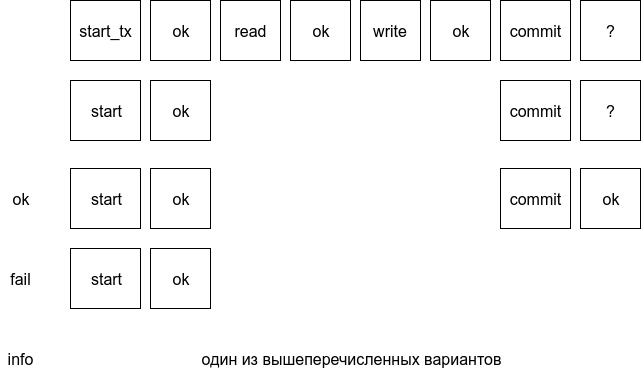
\includegraphics[scale=0.5]{history-transform.png}
    \caption{Преобразование истории. Каждая транзакция  в зависимости от
        статуса завершения может быть несколькими вариантами преобразована в две операции --
        чтения и записи соответственно.}
\end{figure}

\begin{itemize}
    \item Если $commit$ операция завершилась \textbf{fail}-записью, обе записи
        соответствующие $commit$ операции удаляются.
        $start$ операция преобразуется в $read$ операцию для того-же множества регистров.
        То есть не меняющее состояние объекта чтение.
    \item Если $commit$ операция завершилась \textbf{ok}-записью, то
        $start$-операция преобразуется в $read$ операцию, блокирующую регистры,
        в которые пишет $commit$ операция. Соответственно операция определена только на объектах,
        в которых соответствующие регистры не заблокированы. $commit$ операция преобразуется в
        $write$ операцию, при этом разблокирующую регистры в которые пишет.
        Соответственно определена только на объектах, в которых соответствующие регистры заблокированы.
    \item Если $commit$ операция не завершилась или завершилась \textbf{info}-записью, то рассматриваем два варианта истории,
        преобразованной одним из вышеупомянутых способов.
\end{itemize}

Таким образом получаем некоторое множество историй.
\begin{lemma}
    Snapshot-сериализуемость исходной истории равносильна линеаризуемости одной из историй, полученных
    приведённым преобразованием.
\end{lemma}
\begin{proof}
    В одну из сторон приведённое утверждение очевидно. То есть из snapshot-сериализуемости очевидна линеаризуемость
    одной из полученных историй. Пусть $T$ получена из $H$ и $L$ -- линеаризация $T.$ Покажем как построить линеаризацию
    $H$ удовлетворяющую \ref{snapshot-def}. Рассмотрим $L'$ соответствующую $L.$ В том смысле, что операции в $L'$ получаются
    из операций в $L$ игнорированием блокировки регистров. $read$-записям соответствуют $start$-записи,
    $write$ переходят в $commit$. Рассмотрим ограничение $L$ на один из регистров. Также удалим неблокирующие чтения.
    Из линеаризуемости $T$ очевидно, что чтения и записи чередуются, и история начинается с чтения.
    Покажем, что история устроена следующим образом: каждой записи предшествует соответствующее чтение(с тем же идентификатором
    процесса), устанавливающее блокировку и за каждым чтением следует соответствующая запись. От противного: пусть пара $u$, $v$
    -- последовательные чтение и запись с разными идентификаторами процесса. Тогда в истории должно присутствовать соответствующее
    $v$ чтение $w$. Более того, оно должно быть расположено перед $u.$ Тогда после него должна быть запись с другим идентификатором
    процесса. Получаем противоречие с тем что пара $u, v$ первая. Пусть теперь пара $u$, $v$ в $L'$ -- соответствующие $start$ и
    $commit$ операции. Пусть между $u$ и $v$ есть $w$ которая пишет в один из регистров, в которые пишет $v.$ Тогда ограничивая $L$ на
    этот регистр получаем противоречие вышедоказанному.
\end{proof}

Алгоритм устроен следующим образом:
\begin{itemize}
    \item Сначала строится преобразование истории: при неоднозначности преобразования элементом истории является кортеж альтернатив.
        У $ret$-записей альтернатив нет. Для некоторых записей помечаем что при выполнении следующую операцию
        данного процесса надо игнорировать.
    \item Удаляются все \textbf{fail} и \textbf{info} записи. Для \textbf{fail}-записей необходимо удалить также \textbf{call}-запись.
    \item Производится поиск в пространстве состояний, схожий с описанным в разделе \ref{cypress-verify}.
\end{itemize}

Состоянием так же является $\langle state, history \rangle.$
При вычислении смежных состояний мы рассматриваем все альтернативы для каждой \textbf{call}-записи, и удаляем
из истории следующую операцию процесса(если помечено что надо её проигнорировать).
При поиске запоминаем пройденные состояния, в том смысле что запоминаем пару (множество удалённых операций, состояние).
В \cite{horn-faster} запоминали именно пару $\langle state, history \rangle,$ что создавало некоторое замедление из-за
необходимости сравнения историй, которые хранились в неизменяемом односвязном списке. Авторы предлагают кешировать результаты
сравнения списков для ускорения работы алгоритма. Мы же, поддерживая множество удалённых операций(bitset) добились сравнимой
производительности при меньшей сложности алгоритма.

Как и в алгоритме, описанном в \ref{cypress-verify}, при постановке экспериментов,
перед началом работы алгоритма явно строится граф состояний и переходов для модели,
мемоизируется именно множество удалённых операций, но в отличие от \cite{knossos}, мы
используем неизменяемые списки, что с одной стороны замедляет алгоритм, но с другой позволяет
эффективно распределить вычисления на несколько процессорных ядер и результирующее время работы
(на синтетических тестах) получается меньше.

\begin{center}
  \begin{tabular}{| c | c | c | c | c| }
      \hline
        Номер теста & Длина истории & knossos & наша реализация \\
        \hline
        1           & 20            & 0.2с     & 2с             \\
        \hline
        2           & 200           & 40с      & 10с              \\
        \hline
        3           & 800           & 1200с    & 100с              \\
        \hline
  \end{tabular}
\end{center}
Все тесты производились на 16-ядерном процессоре, с доступным объёмом памяти 60G.

\end{document}
